\begin{titre}[Fonctions de référence]

\Titre{La fonction Cube}{3}
\end{titre}

\begin{CpsCol}
\textbf{Variations de fonctions}
\begin{description}
\item[$\square$] Connaitre la fonction Cube : définition et courbes représentative.
\item[$\square$] Pour la fonction Cube, résoudre graphiquement ou algébriquement une équation ou une inéquation du type $f(x) = k$, $f(x) < k$.
\item[$\square$] Étudier la parité d'une fonction dans des cas simples.
\end{description}
\end{CpsCol}




\begin{DefT}{Fonction Cube}\index{Fonctions!Cube}
La \textbf{fonction Cube} $f$ est la fonction définie sur $\R$ par $f(x)=x^3$.
\end{DefT}

 
\begin{DefT}{Racine cubique}\index{Fonctions!Racine cubique}
La \textbf{racine cubique} de $x$ est le \textit{nombre réel} $a$ tel que $a^3=x$. On note : $a = \sqrt[3]{x}$.
\end{DefT}

\begin{Ex}
\begin{description}
\item[•] La  racine cubique  de $8$ est égale à 2, on écrit que $2 = \sqrt[3]{8}$ ou $2^3 = 8$.
\item[•] La  racine cubique  de $-27$ est égale à $-3$, on écrit que $-3 = \sqrt[3]{-27}$ ou $(-3)^3 = -27$.
\end{description}
\end{Ex}



\begin{Pp}[Variations]
\begin{minipage}{0.48\linewidth}
La fonction Cube est strictement  croissante sur $\R$. La fonction Cube est impaire. Sa courbe représentative est symétrique par rapport à l'origine du repère.
\end{minipage}
\hfill
\begin{minipage}{0.48\linewidth}
\begin{tikzpicture}
\tkzTabInit[lgt=1,espcl=2]{ $x$ / 1,$f $ / 2}
{ $-\infty$ , $+\infty$}
\tkzTabVar{-/$-\infty$ , +/$+\infty$ }
\end{tikzpicture}
\end{minipage}
\end{Pp}

\ROC

\mini{
\EPC{1}{FR-45}{Chercher.}
 
\EPC{1}{FR-46}{Raisonner.}
}{
\EPC{1}{FR-48}{Chercher.}
}


\mini{
\EPC{1}{FR-47}{Représenter.}

\EPC{1}{FR-50}{Représenter. Raisonner. Calculer}
}{
\EPC{1}{FR-49}{Chercher.}

\EPCC{1}{FR-51}{Calculer.}
}





